\section{}

\textbf{Tiempo de lectura:} \{s16-reading-time\}

La traducción entre direcciones virtuales y físicas puede realizarse de
diversas maneras. La forma más extendida es la \textbf{{}paginación},
que no es sino un esquema de gestión de la memoria que permite que el
espacio de direcciones físico de un proceso no sea continuo, evitando el
problema de la \textbf{fragmentación externa}.

\section{Método básico}\label{_muxe9todo_buxe1sico}

En la paginación la memoria física se divide en bloques de tamaño fijo
denominados \textbf{marcos}{}, mientras que el espacio de direcciones
virtual se divide en bloques del mismo tamaño que los marcos,
denominados \textbf{páginas}{}. Cuando un proceso va a ser ejecutado,
sus páginas son cargadas desde el almacenamiento secundario en marcos
libres de la memoria física.

\begin{figure}
\centering
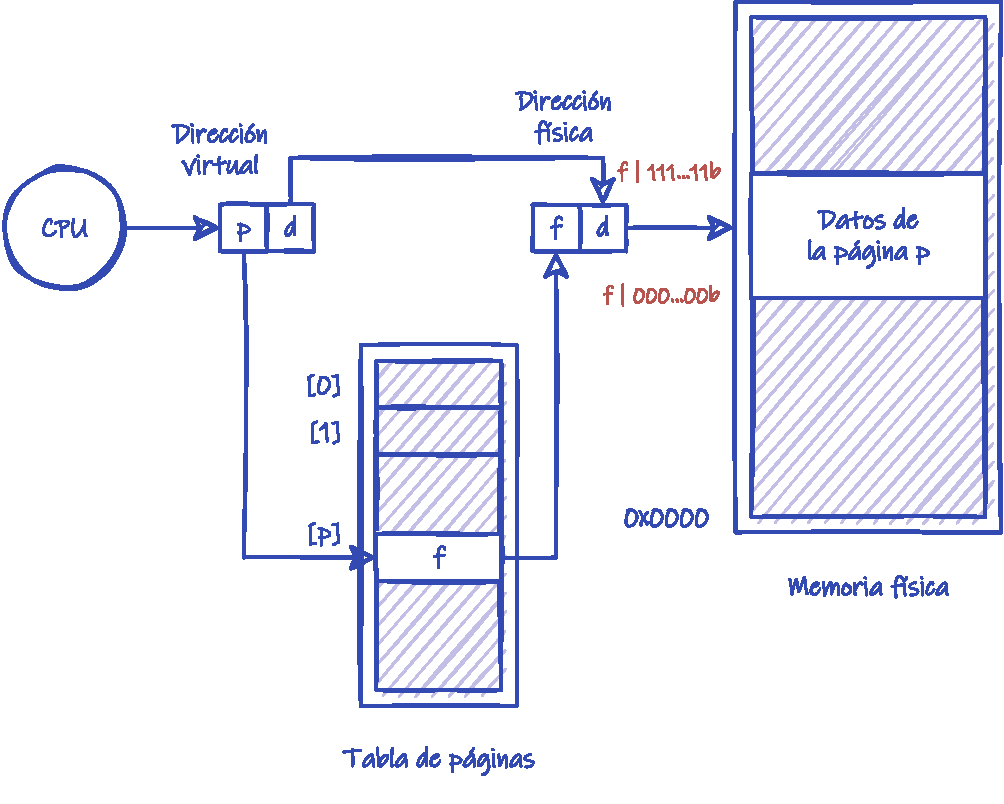
\includegraphics[width=0.8\textwidth]{media/C16_paginación/paginación.pdf}
\caption{Soporte del hardware para la
paginación.}\label{fig-paginaciuxf3n}
\end{figure}

La paginación es una forma de \textbf{reubicación de las direcciones en
tiempo de ejecución} donde la transformación de las direcciones
virtuales en direcciones físicas se realiza de la siguiente manera
(véase la \hyperref[fig-paginaciuxf3n]{Soporte del hardware para la
paginación.}):

\begin{enumerate}
\def\labelenumi{\arabic{enumi}.}
\item
  Cada dirección virtual generada por la CPU es divida en dos partes: un
  \textbf{número de página} \emph{p} y un \textbf{desplazamiento}
  \emph{d}.
\item
  El \textbf{número de página}{} es utilizado por la MMU para indexar la
  \textbf{tabla de páginas}{}, que contiene el \textbf{número de marco}
  \emph{f} de cada \textbf{página} en la memoria física.
\item
  El \textbf{número de marco}{} \emph{f} es combinado con el
  \textbf{desplazamiento} \emph{d} para generar la dirección física que
  va a ser enviada por el bus de direcciones hacia la memoria.
\end{enumerate}

El tamaño de las \textbf{páginas} ---y el de los \textbf{marcos}---
viene definido por el hardware y normalmente es un número entero
potencia de 2 que puede variar entre 512 bytes y 16 MiB, dependiendo de
la arquitectura. Es decir, si el espacio de direcciones es de
2\textsuperscript{\emph{m}} y el tamaño de página es de
2\textsuperscript{\emph{n}}, los \emph{m} - \emph{n} bits de mayor orden
de las direcciones virtuales indican el \textbf{número de página},
mientras que los \emph{n} bits de menor orden indican el
\textbf{desplazamiento} (véase la
\hyperref[fig-direcciuxf3n-virtual-paginaciuxf3n]{Descomposición de las
direcciones virtuales en paginación.}).

\begin{figure}
\centering
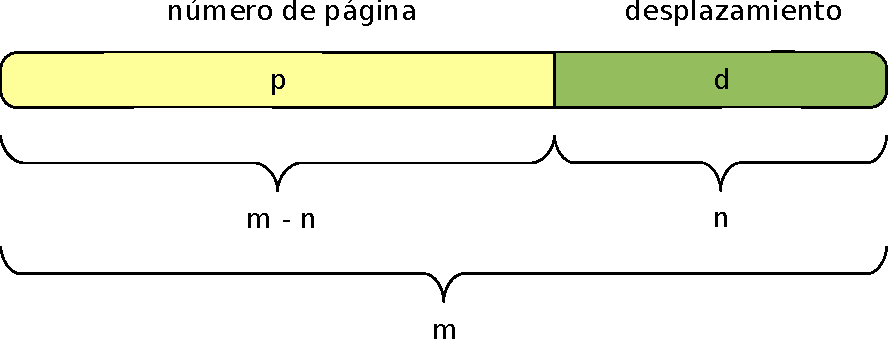
\includegraphics[width=0.8\textwidth]{media/C16_paginación/dirección_virtual_paginación.pdf}
\caption{Descomposición de las direcciones virtuales en
paginación.}\label{fig-direcciuxf3n-virtual-paginaciuxf3n}
\end{figure}

Por ejemplo, en muchos sistemas operativos el tamaño de página es de 4
KiB, por lo que el desplazamiento \emph{n} necesita:

\[n = log_2 4096 = 12\ "bits"\]

Si las direcciones virtuales son de 32 bits, eso deja para el número de
página \emph{p}:

\[p = 32 - 12 = 20\ "bits"\]

por lo que el espacio de direcciones virtual tiene 2\textsuperscript{20}
páginas ---es decir, 1 048 576 páginas---.

\subsection{Desde el punto de vista de los
procesos}\label{_desde_el_punto_de_vista_de_los_procesos}

Cada \textbf{página} de un proceso requiere un \textbf{marco}. Por
tanto, cuando un proceso llega al sistema:

\begin{enumerate}
\def\labelenumi{\arabic{enumi}.}
\item
  Si el proceso requiere \emph{n} \textbf{páginas}, el sistema operativo
  debe escoger \emph{n} \textbf{marcos}. Estos \textbf{marcos} son
  tomados de la \textbf{lista de marcos libres}{} que debe mantener el
  sistema. Puesto que son escogidos de allí donde los haya libres, el
  \textbf{espacio de direcciones físico} puede no ser contiguo, aunque
  los procesos vean un \textbf{espacio de direcciones virtual} contiguo.
\item
  Los \textbf{marcos} seleccionados son asignados al proceso y cada
  \textbf{página} del proceso es cargada en uno de dichos
  \textbf{marcos}.
\item
  La \textbf{tabla de páginas} es actualizada de manera que en la
  entrada de cada \textbf{página} del proceso se pone el número de
  \textbf{marco} correspondiente.
\end{enumerate}

Un aspecto importante de la paginación es la diferencia entre cómo ven
los procesos la memoria y como es realmente la memoria física. Cada
proceso ve la memoria como un espacio único que lo contiene solo a él.
Sin embargo, la realidad es que el programa está disperso por la memoria
física, que además puede almacenar a otros programas. Esto es posible
porque en cada momento la \textbf{tabla de páginas} solo contiene las
\textbf{páginas} del proceso en ejecución en la CPU.

\subsection{Desde el punto de vista del sistema
operativo}\label{_desde_el_punto_de_vista_del_sistema_operativo}

Puesto que el sistema operativo es quién gestiona la memoria física,
este debe saber:

\begin{itemize}
\item
  Que \textbf{marcos} están asignados y a que \textbf{página} de qué
  proceso o procesos.
\item
  Que \textbf{marcos} están disponibles.
\end{itemize}

Toda esta información generalmente se guarda en una estructura
denominada la \textbf{tabla de marcos}{}, que tiene una entrada por cada
\textbf{marco} de la memoria física.

Además, el sistema operativo debe mantener una copia de la \textbf{tabla
de páginas} para cada proceso en el \textbf{PCB}, igual que mantiene una
copia del contador de programa y del contenido de los registros de la
CPU. Esta copia es utilizada:

\begin{itemize}
\item
  Por el \textbf{asignador} para sustituir la \textbf{tabla de páginas}
  usada por la CPU cuando realiza un \textbf{cambio de contexto}. Por lo
  tanto, el uso de la paginación incrementa el tiempo del cambio de
  contexto.
\item
  Para la traducción manual de direcciones virtuales en físicas. Por
  ejemplo, cuando un proceso realiza una llamada al sistema para
  realizar una operación de E/S y proporciona una dirección como
  parámetro, dicha dirección debe ser traducida manualmente para
  producir la dirección física correspondiente, que será comunicada al
  hardware para realizar la operación.
\end{itemize}

\subsection{Tamaño de las páginas}\label{_tamauxf1o_de_las_puxe1ginas}

Una decisión de diseño importante es escoger el tamaño de las
\textbf{páginas} adecuado:

\begin{itemize}
\item
  Con \textbf{páginas} más pequeñas esperamos tener menos
  \textbf{fragmentación interna}.
\item
  Con páginas más grandes se pierde menos espacio en la \textbf{tabla de
  páginas}. No olvidemos que cuanto más pequeñas son las
  \textbf{páginas}, más \textbf{páginas} son necesarias y, por tanto,
  más entradas en la \textbf{tabla de páginas} se necesitan. Además, la
  E/S es más eficiente cuanto más datos son transferidos de cada vez.
\end{itemize}

Los tamaños de \textbf{páginas} típicos son 4 y 8 KiB. En un sistema de
32 bits con páginas de 4 KiB ---como del que hablamos antes--- el
espacio de direcciones virtual tiene 1 048 576 páginas. Si se utilizan 4
bytes para cada entrada de la \textbf{tabla de páginas} ---aunque esto
también puede variar--- eso significa que cada \textbf{tabla de páginas}
ocupa 4 MiB de espacio. Mientras que con \textbf{páginas} de 8 KiB, la
\textbf{tabla de páginas} ocuparía 2 MiB de espacios.

También significa que si los 4 bytes de la \textbf{tabla de páginas} se
utilizan para guardar únicamente el \textbf{número de marco}, cada
entrada puede direccionar a uno de 2\textsuperscript{32} ---o 4 GiB---
\textbf{marcos} de la memoria física. Si el tamaño de cada
\textbf{marco} es de 4 KiB ---dado que debe coincidir con el tamaño de
las páginas--- podemos determinar que el sistema es capaz de direccionar
2\textsuperscript{44} bytes ---o 16 TiB--- de memoria física, aunque el
espacio de direcciones virtual de cada proceso solo le da acceso a un
máximo de 4 GiB.

\section{Soporte hardware de la tabla de
páginas}\label{_soporte_hardware_de_la_tabla_de_puxe1ginas}

La implementación en hardware de la \textbf{tabla de páginas} puede
realizarse de diversas maneras.

\subsection{Almacenada en registros de la
CPU}\label{_almacenada_en_registros_de_la_cpu}

La \textbf{tabla de páginas} del proceso actual en la CPU puede alojarse
dentro de la propia CPU, en unos registros destinados a tal fin.

Debido a la velocidad de los registros de la CPU, la implementación en
registros es la más eficiente. Sin embargo, solo puede ser utilizado
para \textbf{tablas de páginas} razonablemente pequeñas, ya que alojar
tablas de más de 256 entradas en registros es muy costoso.

Por ejemplo, el DEC \href{https://es.wikipedia.org/wiki/PDP-11}{PDP-11}
---para el que se diseñó el primer UNIX--- es un ejemplo de sistema con
esta implementación. Utilizaba un espacio de direcciones de 16 bits y un
tamaño de \textbf{páginas} de 8 KiB, por lo que solo necesitaba 8
registros dedicados para alojar toda la \textbf{tabla de páginas}.

\subsection{Almacenada en memoria}\label{_almacenada_en_memoria}

La otra opción es alojar la \textbf{tabla de páginas} del proceso actual
en la memoria, normalmente en un formato definido por la CPU.

En los sistemas modernos se utilizan \textbf{tablas de páginas} de un
millón de entradas o más, que difícilmente pueden alojarse en registros
dentro de la CPU. Por eso, los sistemas actuales almacenan la
\textbf{tabla de páginas} del proceso actualmente en ejecución, en la
memoria. Eso permite disponer de \textbf{tablas de páginas} de gran
tamaño, aunque a costa de necesitar dos accesos a la memoria física por
cada acceso a una dirección virtual.

Para que la MMU pueda conocer la ubicación de la \textbf{tabla de
páginas} durante la traducción de las direcciones, la CPU debe disponer
de un registro ---el \textbf{{}PTBR} (\emph{Page-Table Base
Register})--- donde se guarda la dirección de la \textbf{tabla de
páginas} actual.

Además, esto tiene la ventaja de que el \textbf{cambio de contexto} es
más rápido ---respecto al uso de registros para almacenar la tabla de
páginas--- puesto que solo es necesario cargar un único registro más
---el \textbf{PTBR}--- durante el mismo.

\subsection{TLB}\label{_tlb}

La solución al retraso originado por el acceso a la tabla de páginas,
cuando esta está en la memoria, pasa porque el sistema disponga de una
pequeña caché de traducciones en hardware llamada \textbf{{}TLB}
(\emph{Translation Look-aside Buffer}).

La \textbf{TLB} es una memoria asociativa de alta velocidad. Cada
entrada de la \textbf{TLB} tiene dos partes: la \textbf{clave} ---o
etiqueta--- y el valor. Cuando a la \textbf{TLB} se le entrega un
elemento, este es comparado simultáneamente con todas las claves. Si se
produce alguna coincidencia, la memoria devuelve el valor de la entrada
correspondiente.

Debido a la forma que tienen de operar, son rápidas pero muy caras de
fabricar. Por ello, el número de entradas es bajo, normalmente entre 64
y 1024.

\subsubsection{Uso básico de la TLB}\label{_uso_buxe1sico_de_la_tlb}

La \textbf{TLB} es utiliza con la \textbf{tabla de páginas} de la
siguiente manera:

\begin{figure}
\centering
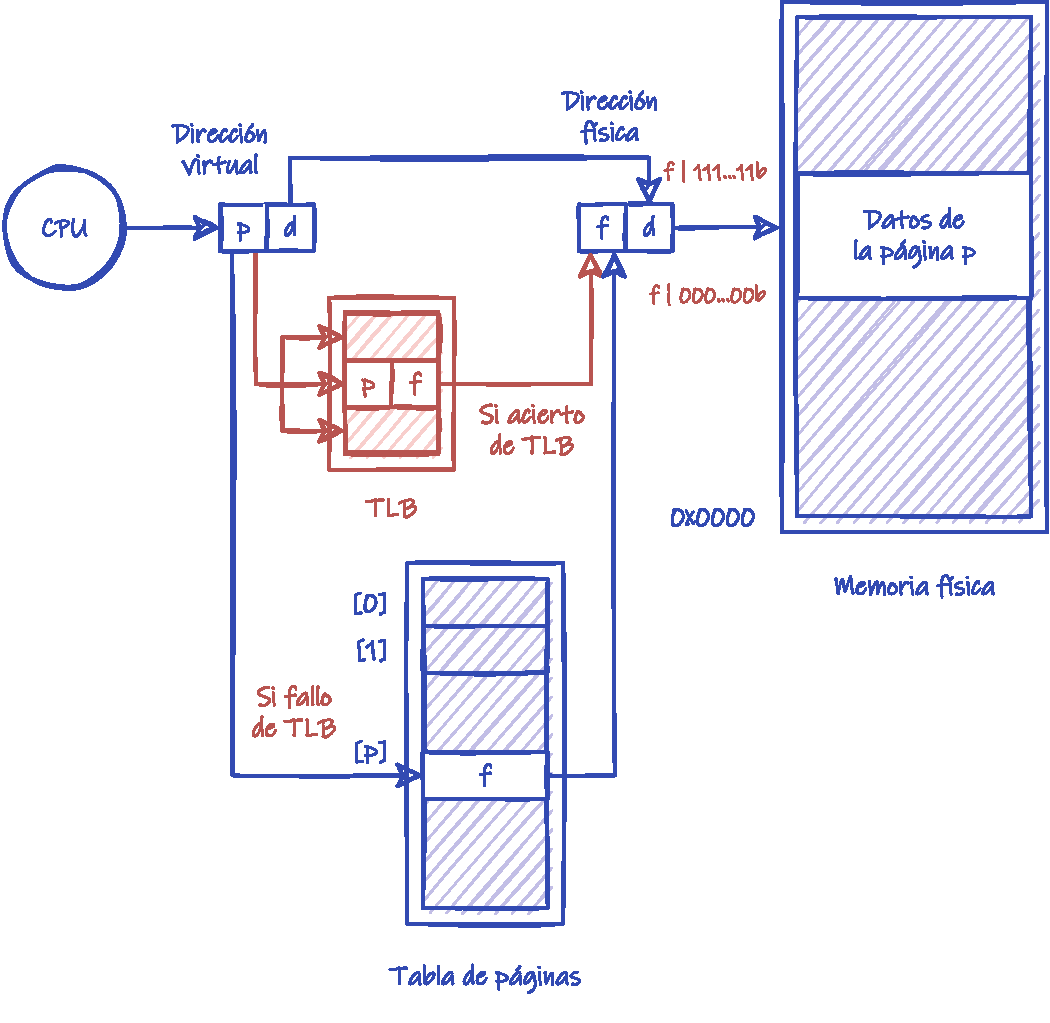
\includegraphics[width=0.8\textwidth]{media/C16_paginación/tlb.pdf}
\caption{Soporte del hardware para la paginación con
TLB.}\label{fig-paginaciuxf3n-tlb}
\end{figure}

\begin{enumerate}
\def\labelenumi{\arabic{enumi}.}
\item
  La \textbf{TLB} contiene unas pocas entradas de la \textbf{tabla de
  páginas}.
\item
  Cuando la CPU genera una dirección virtual, el \textbf{número de
  página} es entregado a la \textbf{TLB}. La \textbf{TLB} utiliza los
  números de páginas como \textbf{clave}, por lo que si hay alguna
  coincidencia, devolverá la entrada correspondiente de la \textbf{tabla
  de páginas}.
\item
  Si hay coincidencia ---o \textbf{acierto de TLB}--- el \textbf{número
  de marco} es extraído de la entrada devuelta por la \textbf{TLB} y es
  utilizado para generar la dirección física. Todo este proceso puede
  requerir un 10\% más de tiempo que si no se hiciera la traducción de
  las direcciones.
\item
  Si no hay coincidencia ---o \textbf{fallo de TLB}--- es necesario
  acceder a la \textbf{tabla de páginas} para obtener la entrada
  correspondiente directamente de ella. Indudablemente, este acceso
  puede beneficiarse de la existencia de diferentes niveles de caché en
  el acceso a la memoria principal.
\item
  En este último caso, la entrada recuperada debe ser añadida a la
  \textbf{TLB}, por lo que sí está llena, se debe seleccionar una para
  ser sustituida. Los algoritmos de reemplazo utilizados van, desde
  elegir una aleatoriamente, hasta el \textbf{{}LRU} (\emph{Least
  Recently Used}).
\end{enumerate}

\subsubsection{Borrado de la TLB en el cambio de
contexto}\label{_borrado_de_la_tlb_en_el_cambio_de_contexto}

Una cuestión importante es qué ocurre con las \textbf{TLB} cuando el
sistema operativo realiza un \textbf{cambio de contexto}.

En general, es necesario que el asignador realice un borrado de la
\textbf{TLB}. De lo contrario, el nuevo proceso podría utilizar las
entradas de la \textbf{tabla de páginas} del viejo proceso, que
estuvieran almacenadas en la \textbf{TLB}. Sin embargo, un proceso no
tiene por qué utilizar todas las entradas de la \textbf{TLB}, por lo que
sería más interesante, no tener que borrar las entradas de procesos
anteriores, mientras no sean necesarias, por si estos vuelven a ser
ejecutados en la CPU.

El borrado se puede evitar si cada entrada de la \textbf{TLB} tiene un
\textbf{{}ASID} (\emph{Address-Space Identification}), que no es más que
un identificador único para cada proceso. En este tipo de \textbf{TLB},
en la \textbf{clave} se buscan pares \textbf{(número de página, ASID)},
donde el primero proviene de la dirección virtual y el segundo es el
\textbf{ASID} del proceso actual. De esta forma, si el \textbf{número de
página} coincide, pero no el \textbf{ASID}, se produce un fallo de la
\textbf{TLB}. Esto obliga a acceder a la \textbf{tabla de páginas} en
memoria para recuperar la entrada, evitando que se lea por error la
entrada de un proceso anterior.

Esta característica está presente en los procesadores \{decalpha\},
\{mips\} y \{ultrasparc\}. Entre 2005 y 2006 también comenzó a ser
incluida en algunos procesadores de la familia x86, a través de las
extensiones de virtualización Intel VT y AMD Pacifica.

\section{Tiempos de acceso a la
memoria}\label{_tiempos_de_acceso_a_la_memoria}

El rendimiento de un sistema con paginación, está relacionado con el
concepto de \textbf{tiempo de acceso efectivo}{} a la memoria
\(T_text(em)\), que intenta estimar el tiempo que realmente se tarda en
acceder a la memoria, teniendo en cuenta mecanismos del sistema
operativo como el método de paginación o la existencia de \textbf{TLB}.

En muchos sistemas informáticos, el \textbf{tiempo de acceso}{} a la
memoria física \(T_text(m)\) es de unos pocos nanosegundos. Por tanto,
en el método de básico de paginación ---con una \textbf{tabla de páginas
lineal}{}--- y sin \textbf{TLB}, el \textbf{tiempo de acceso efectivo}
\(T_text(em)\) es el doble del \textbf{tiempo de acceso} \(T_text(m)\) a
la memoria:

\[T_text(em)=2T_text(m)\]

porque es necesario acceder a la memoria en dos ocasiones:

\begin{enumerate}
\def\labelenumi{\arabic{enumi}.}
\item
  Primero, para consultar la \textbf{tabla de páginas}, con el objetivo
  de traducir la dirección virtual en una dirección física.
\item
  Después, para realizar la operación solicitada sobre la memoria
  física.
\end{enumerate}

Obviamente, en métodos de paginación donde hagan falta más accesos para
obtener finalmente el \textbf{número de marco}, el \textbf{tiempo de
acceso efectivo} será mayor.

En el caso anterior, el segundo acceso a la memoria es inevitable,
porque corresponde a la operación solicitada por el proceso. Mientras
que el primero puede evitarse, en ciertas ocasiones, consultado la
\textbf{TLB} antes de acceder a la \textbf{tabla de páginas}. Es decir,
en un sistema con \textbf{TLB}:

\begin{itemize}
\item
  Cuando la dirección virtual \textbf{NO} está en la \textbf{TLB}:
  \(T_text(em)=2T_text(m) + T_text(TLB)\), porque primero se accede a la
  \textbf{TLB} y después ---como no se encuentra allí la direcció
  virtual--- se consulta la \textbf{tabla de páginas}.
\item
  Cuando la dirección virtual está en la \textbf{TLB}:
  \(T_text(em)=T_text(m) + T_text(TLB)\), porque la \textbf{TLB}
  proporciona la información necesaria para traducir la dirección,
  evitando la consulta posterior a la \textbf{tabla de páginas}.
\end{itemize}

El cálculo de \(T_text(em)\) puede complicarse aun más si tenemos en
cuenta que los sistemas suelen tener varios niveles de memoria caché. En
ese caso \(T_text(m)\) no tiene un valor determinado, sino que se estima
un promedio considernado tanto el tiempo de acceso a la memoria física
como a cada uno de los niveles de caché del sistema, así como la
probabilidad de que la dirección de memoria a la que se quiere acceder
esté disponible en alguno de dichos niveles.

El \(T_text(em)\) del primer caso suele ser mucho mayor que el segundo
porque, por lo general, \(T_text(TLB) ll T_text(m)\). Esto hace que en
muchos sistemas se pueda considerar que \(T_text(em) ~~ T_text(m)\)
cuando la dirección virtual está en la \textbf{TLB}.

Como el \textbf{tiempo de acceso efectivo} \(T_text(em)\) ahora depende
de la probabilidad \(p_text(TLB)\) de que las direcciones virtuales
consultadas estén en la \textbf{TLB}, ya no podemos hacer el cálculo de
forma determinista, sino estimar un \(T_text(em)\) promedio para el
sistema. Para ello, solo es necesario sumar el \(T_text(em)\) para ambos
casos, ponderando por la probabilidad \(p_text(TLB)\) de que la
dirección esté en la \textbf{TLB} o \((1 - p_text(TLB))\) de que no esté
en la \textbf{TLB}, respectivamente:

\[{:(T_"em", =, (1-p_"TLB")*(2T_"m" + T_"TLB") + p_"TLB"*(T_"m" + T_"TLB")),
    (    , =, (2-p_"TLB")*T_"m" + T_"TLB"\qquad\qquad\qquad\qquad\qquad\ \ \ ):}\]

Como comentamos anteriormente, esta expresión se puede simplificar si
consideramos que \(T_text(TLB) ll T_text(m)\):

\[{:(T_"em", =, 2*(1-p_"TLB")*T_"m" + p_"TLB"*T_"m"),
    (    , =, (2-p_"TLB")*T_"m"\qquad\qquad\qquad\ \ \ ):}\]

Obviamente, cuanto más se aproxima a 1 la probabilidad \(p_text(TLB)\)
de que la entrada esté en la \textbf{TLB}, más cerca está \(T_text(em)\)
de \(T_text(m)\).

Para mejorar esta probabilidad:

\begin{itemize}
\item
  Las \textbf{TLB} permiten marcar algunas entradas como insustituibles.
  Esto normalmente se hace con las entradas de las \textbf{páginas} del
  código y los datos del núcleo, ya que son páginas que se utilizan con
  muchísima frecuencia.
\item
  Si la MMU soporta páginas de mayor tamaño que el estándar, se utilizan
  para alojar el código y los datos del núcleo. De esta forma se
  minimiza el número de entradas de la \textbf{TLB} que utilizan, con el
  fin de disponer de más entradas libres para los procesos en ejecución.
\end{itemize}

En la familia x86 el tamaño de página estándar es de 4 KiB, pero también
se puede disponer de páginas de 4 MiB. En x86-64 las páginas de gran
tamaño son de 2 MiB, aunque algunos modelos también soportan páginas de
1 GiB.

\section{Protección de la memoria}\label{_protecciuxf3n_de_la_memoria}

La protección de las páginas se consigue mediante unos bits que indican
las operaciones que se pueden realizar sobre ellas. Normalmente, estos
bits son almacenados en cada una de las entradas de la \textbf{tabla de
páginas}.

\subsection{Bits de protección}\label{_bits_de_protecciuxf3n}

{} Los \textbf{bits de protección} pueden ser:

\begin{itemize}
\item
  \textbf{Solo lectura}.
\item
  \textbf{Lectura --- Escritura}. En algunos sistemas hay un bit
  específico para este permiso, mientras que en otros se utilizan bits
  separados, como: \textbf{lectura}, \textbf{escritura} y
  \textbf{ejecución}; que se pueden combinar libremente.
\item
  \textbf{Solo ejecución}. Que no existen en todas las plataformas. Por
  ejemplo, la familia x86 careció de esta característica hasta que AMD
  la incluyó en su arquitectura x86-64, lo que obligó a Intel a
  incluirla en las versiones más modernas de Pentium IV. El bit ---que
  para ser exacto indica \textbf{no ejecución}--- fue introducido para
  evitar cierto tipo de ataques de seguridad.
\end{itemize}

Durante la traducción de las direcciones, la MMU comprueba que el tipo
de acceso sea válido. Si no lo es, se genera una excepción de violación
de protección de memoria, dado que el acceso en un modo no autorizado se
considera una instrucción privilegiada. Normalmente, el sistema
operativo responde a dicha excepción terminando el proceso que la
generó.

\subsection{Bit de válido}\label{_bit_de_vuxe1lido}

{} Además de los \textbf{bits de protección} comentados, se suele añadir
a cada entrada un \textbf{bit de válido}:

\begin{itemize}
\item
  Cuando una \textbf{página es válida}, la página existe en el espacio
  de direcciones virtual del proceso. Es decir, que la página se puede
  utilizar. Otro término comúnmente utilizado, es que la página es
  \textbf{legal}{}.
\item
  Cuando la \textbf{página es inválida}, la página no existe en el
  espacio de direcciones virtual del proceso. Es decir, que la página no
  se puede utilizar. El término alternativo utilizado es que la página
  es \textbf{ilegal}{}.
\end{itemize}

Al igual que con los \textbf{bits de protección}, los intentos de acceso
a una página ilegal generan una excepción.

El sistema operativo puede utilizar este bit para permitir o denegar
cualquier tipo de acceso a una \textbf{página}. Generalmente, porque no
se le ha asignado un \textbf{marco} de memoria física, ya que esa página
no está siendo utilizada por el proceso.

\begin{figure}
\centering
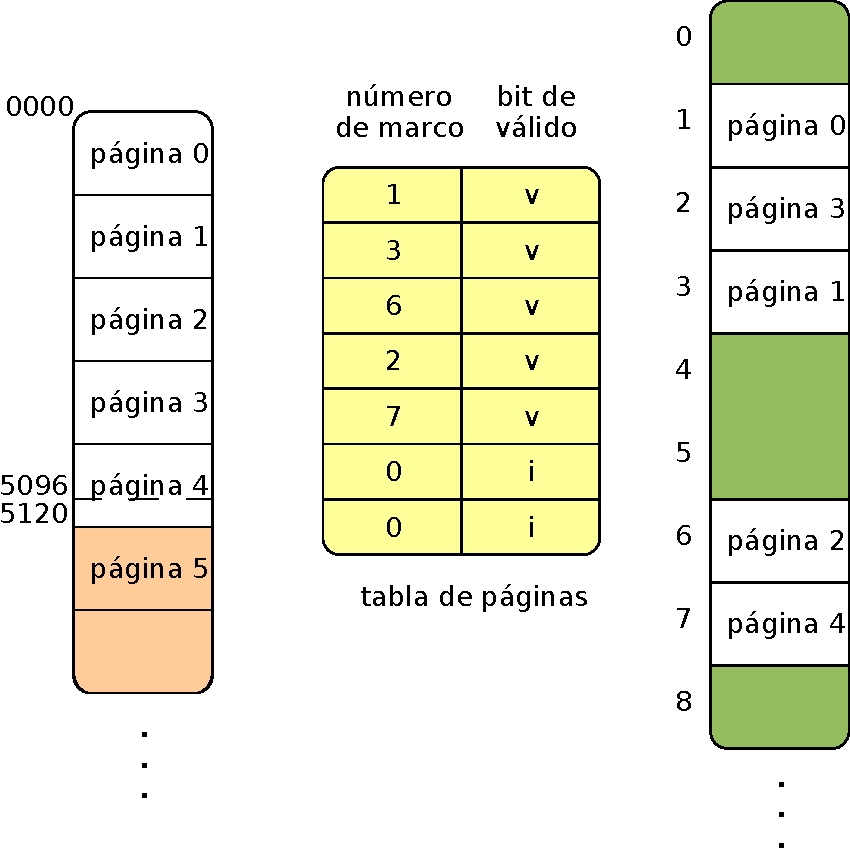
\includegraphics[width=0.8\textwidth]{media/C16_paginación/bit_de_válido_en_la_tabla_de_páginas.pdf}
\caption{Bit de válido en la tabla de
páginas.}\label{fig-bit-de-vuxe1lido-en-la-tabla-de-puxe1ginas}
\end{figure}

Por ejemplo, en la
\hyperref[fig-bit-de-vuxe1lido-en-la-tabla-de-puxe1ginas]{Bit de válido
en la tabla de páginas.}, vemos el espacio de direcciones virtual y la
\textbf{tabla de páginas} de un proceso de 5096 bytes en un sistema con
\textbf{páginas} de 1 KiB. Puesto que el proceso no ocupa todo el
espacio de direcciones, solo las direcciones de la 0 a la 5119 son
válidas. En dicho ejemplo, podemos apreciar varios fenómenos:

\begin{itemize}
\item
  Debido a la \textbf{fragmentación interna}, las direcciones de la 5097
  a la 5119 son válidas, aunque el proceso solo ocupe hasta la 5096. Es
  decir, se está asignando al proceso una porción de memoria que no
  necesita.
\item
  Solo las \textbf{páginas} con datos y código del proceso son válidas.
  Mientras que todas las \textbf{páginas} con direcciones por encima de
  la 5119 están marcadas como ilegales.
\end{itemize}

En general, los procesos solo necesitan una porción muy pequeña de su
espacio de direcciones virtual. Por ejemplo, en un sistema de 32 bits,
muy pocos procesos necesitan los 3 GiB disponibles como máximo para cada
proceso ---el 1 GiB restante suele estar ocupado por el núcleo del
sistema---. Utilizando el \textbf{bit de válido}, el sistema operativo
no tiene que asignar \textbf{marcos} a \textbf{páginas} no utilizadas
por el proceso, ahorrando mucha memoria.

En el \hyperref[_tamauxf1o_de_las_puxe1ginas]{Tamaño de las páginas},
vimos que el tamaño de la \textbf{tabla de páginas} se puede calcular
como el número máximo de páginas del espacio de direcciones virtual
multiplicado por el tamaño de cada entrada de la tabla. Así, en un
sistema de 32 bits con páginas de 4 KiB y 4 bytes por entrada, se
necesitan 4 MiB de memoria para almacenar la \textbf{tabla de páginas}.
Como un proceso suele ocupar muy poco de su espacio de direcciones
virtual, suele ser un desperdicio de memoria crear y almacenar una
\textbf{tabla de páginas} completa, con una entrada para cada
\textbf{página} del espacio de direcciones.

Para evitarlo, en algunas CPU existe el registro \textbf{{}PTLR}
(\emph{Page-Table Length Register}) que se utiliza para indicar el
tamaño actual de la \textbf{tabla de páginas}. Este valor es comparado
por la MMU, durante la traducción de las direcciones virtuales, con el
\textbf{número de página} de cada dirección virtual, de manera que las
\textbf{páginas} con entradas más allá de la última almacenada en la
tabla son consideradas ilegales.

\begin{figure}
\centering
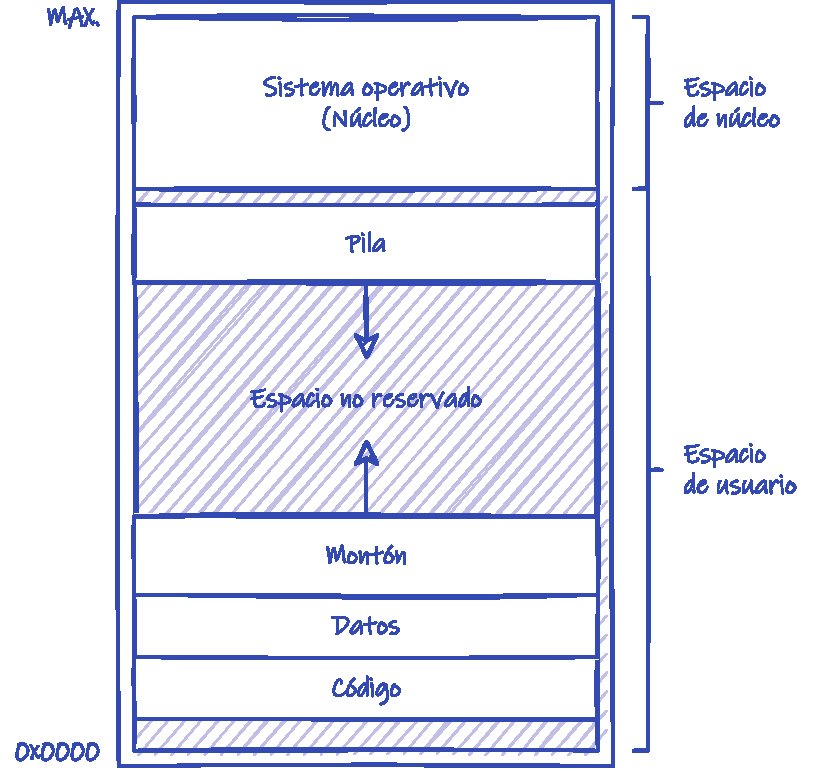
\includegraphics[width=0.8\textwidth]{media/C16_paginación/proceso_en_memoria.pdf}
\caption{Anatomía de un proceso en
memoria.}\label{fig-proceso-en-memoria-disperso}
\end{figure}

En realidad, el registro \textbf{PTLR} no es de mucha utilidad en los
sistemas operativos modernos porque, tal y como vimos en el
\hyperref[_el_proceso]{???}, lo más común es que los procesos tengan un
espacio de direcciones virtual disperso como el de la
\hyperref[fig-proceso-en-memoria-disperso]{Anatomía de un proceso en
memoria.}. En ella, podemos observar, como el sistema operativo ubica
los diferentes componentes del proceso de una forma particular dentro
del espacio de direcciones virtual. Este esquema permite que tanto el
\textbf{montón} ---a través del mecanismo de asignación dinámica de
memoria--- como la \textbf{pila} puedan extenderse ---según las
necesidades de memoria que tenga el proceso--- sobre la región de
memoria no ocupada. Esa región también puede ser parcialmente ocupada
por \textbf{librerías de enlace dinámico} o regiones de \textbf{memoria
compartida}, si son necesarias durante la ejecución del proceso.

En cualquier caso, las \textbf{páginas} de la región no ocupada, forman
parte del espacio de direcciones virtual, pero no necesitan tener
asignado ningún \textbf{marco} de memoria física, en tanto en cuanto el
proceso no las vaya a utilizar. La falta de \textbf{marco} es indicada
por el sistema operativo utilizando el \textbf{bit de válido} para
denegar el acceso.

\section{Páginas compartidas}\label{_puxe1ginas_compartidas}

{} Una de las ventajas importantes de la paginación, es la posibilidad
de compartir \textbf{páginas} entre procesos. Para conseguir esto, basta
con que las \textbf{páginas compartidas} de los distintos procesos
tengan asignadas un mismo \textbf{marco}. Esto permite, por ejemplo, que
los procesos de un mismo programa puedan compartir las \textbf{páginas}
de código o los datos de solo lectura con el fin de ahorrar memoria.
También permite compartir las \textbf{páginas} de código de una librería
compartida enlazada en diferentes procesos.

Compartir \textbf{páginas} no solo permite ahorrar memoria, pues en los
sistemas operativos modernos, la comunicación entre procesos mediante
memoria compartida (véase el \hyperref[memoria_compartida]{???}), se
implementa mediante \textbf{páginas compartidas}.

\section{Paginación jerárquica}\label{_paginaciuxf3n_jeruxe1rquica}

{} Al método básico de paginación, se lo conoce como \textbf{tabla de
páginas lineal}{}. Sin embargo, las CPU comúnmente, utilizan otras
técnicas a la hora de estructurar la \textbf{tabla de páginas}. Una de
las más comunes es la \textbf{paginación jerárquica}, utilizada en los
procesadores de la familia x86 y en ARM, entre otros.

La mayor parte de los sistemas modernos soportan el uso de espacios de
direcciones de gran tamaño. Por ejemplo, supongamos un sistema con un
espacio de direcciones virtual de 32 bits:

\begin{longtable}[]{@{}
  >{\raggedright\arraybackslash}p{(\linewidth - 2\tabcolsep) * \real{0.5000}}
  >{\raggedright\arraybackslash}p{(\linewidth - 2\tabcolsep) * \real{0.5000}}@{}}
\toprule\noalign{}
\endhead
\bottomrule\noalign{}
\endlastfoot
\textbf{tamaño del espacio de direcciones} & = 2\textsuperscript{32} = 4
GiB \\
\textbf{tamaño de página} & = 2\textsuperscript{12} = 4 KiB \\
\textbf{número de páginas} & = 2\textsuperscript{32} /
2\textsuperscript{12} = 2\textsuperscript{32-12} = 2\textsuperscript{20}
= 1 048 576 entradas \\
\end{longtable}

Es decir, que si el tamaño de cada entrada fuera de 4 bytes, la
\textbf{tabla de páginas} de un proceso podría ocupar hasta 4 MiB; que
debe ser alojada en una región continúa del espacio de direcciones
físico, por lo que podría darse el caso de que en algún momento no
hubiera un hueco contiguo lo suficientemente grande. Una forma de
resolver este problema es partir la \textbf{tabla de páginas}, de manera
que no sea necesario asignarle memoria de forma contigua.

\subsection{Paginación jerárquica de dos
niveles}\label{_paginaciuxf3n_jeruxe1rquica_de_dos_niveles}

La \textbf{paginación jerárquica} se basa en la idea de que un vector de
gran tamaño puede ser mapeado en uno más pequeño, que a su vez, puede
ser mapeado en un vector de menor tamaño.

\begin{figure}
\centering
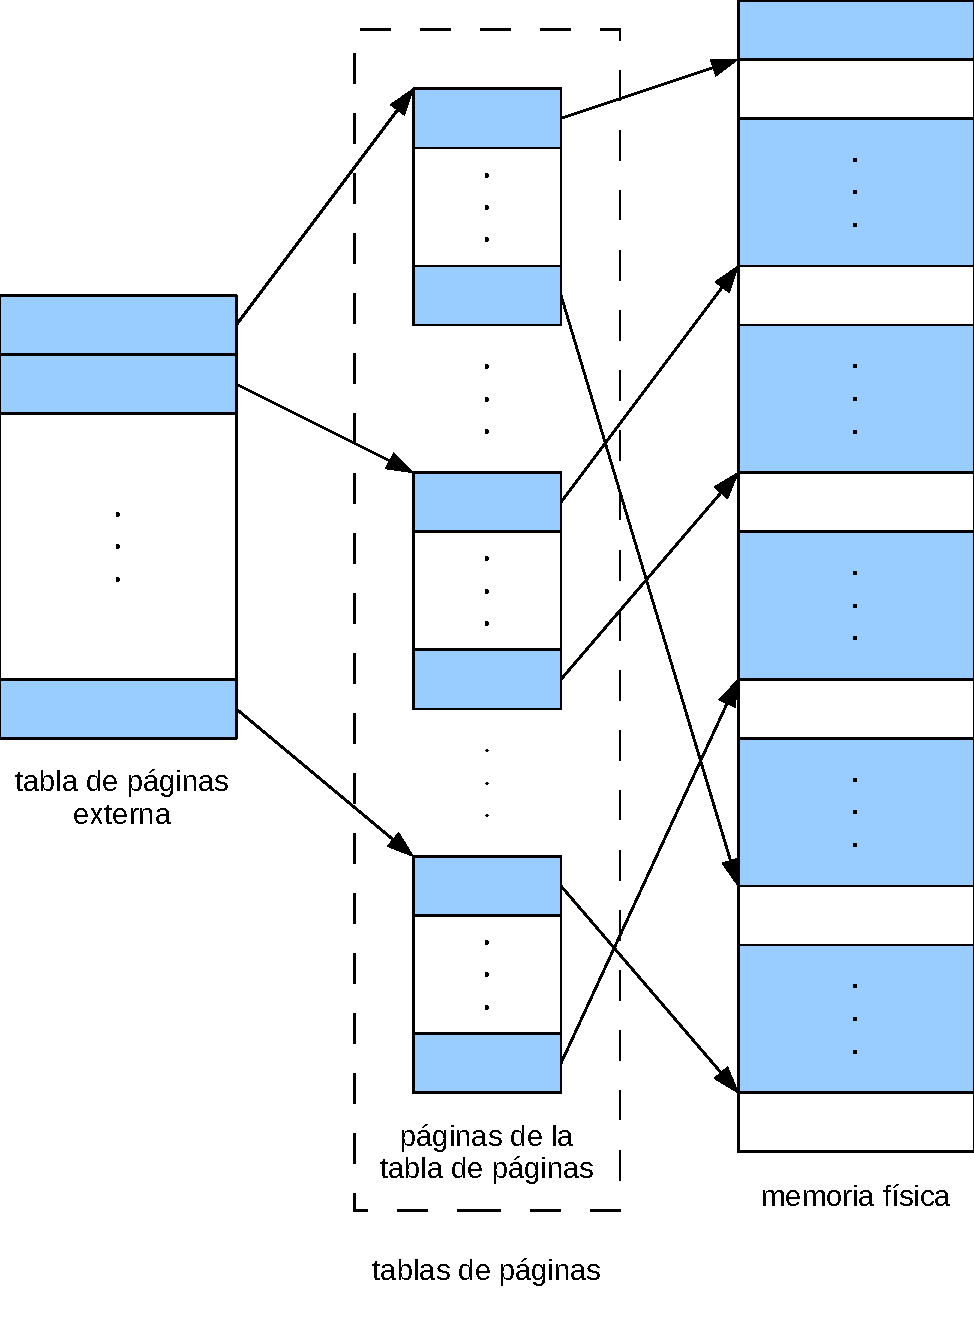
\includegraphics[width=0.8\textwidth]{media/C16_paginación/paginación_jerárquica.pdf}
\caption{Esquema de paginación jerárquica de dos
niveles.}\label{fig-paginaciuxf3n-jeruxe1rquica}
\end{figure}

Por ejemplo, si asumimos el caso anterior de un sistema con un espacio
de direcciones de 32 bits y un tamaño de página de 4 KiB, entonces
podemos dividir la tabla de páginas de 1 048 576 entradas ---4 MiB si
cada entrada necesita 4 bytes--- en 1024 porciones, cada una de las
cuales cabría en un \textbf{marco} de 4 KiB.

Estos \textbf{marcos}, a su vez, pueden ser mapeados por 1024 entradas
con las direcciones físicas de cada \textbf{marco}. Si organizamos estas
1024 entradas en un vector lineal, obtendremos una \textbf{tabla de
páginas externa}{} de 4 KiB (véase la
\hyperref[fig-paginaciuxf3n-jeruxe1rquica]{Esquema de paginación
jerárquica de dos niveles.}).

Dado que 4 KiB es una cantidad de memoria muy pequeña, muchos sistemas
operativos mantienen la \textbf{tabla de páginas externa} en la memoria
mientras el proceso se está ejecutando. Sin embargo, ahora la
\textbf{tabla de páginas} está dividida en \textbf{marcos}, que no
tienen por qué ser asignados de forma contigua en la memoria. Incluso
podrían ser intercambiados al disco, en caso de necesitar memoria libre.

Para tener dos niveles de 1024 entradas, solo es necesario dividir el
\textbf{número de página} \emph{p} de la dirección virtual ---que tenía
2\textsuperscript{20} bits--- en dos \textbf{números de página} de
2\textsuperscript{10} bits cada uno:

\begin{figure}
\centering
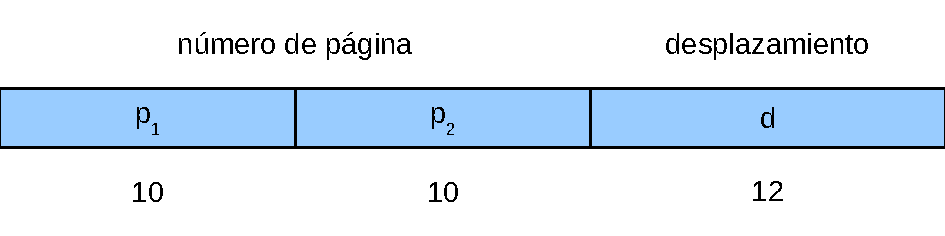
\includegraphics[width=0.8\textwidth]{media/C16_paginación/dirección_virtual_paginación_jerárquica.pdf}
\caption{}
\end{figure}

Este es el método utilizado por la familia de procesadores x86.

Otra variación de la \textbf{paginación jerárquica de dos niveles} es la
utilizada por VAX. Estos sistemas utilizaban una arquitectura de 32 bits
con un tamaño de página de 512 bytes. Las direcciones virtuales eran
divididas de la siguiente manera:

\begin{figure}
\centering
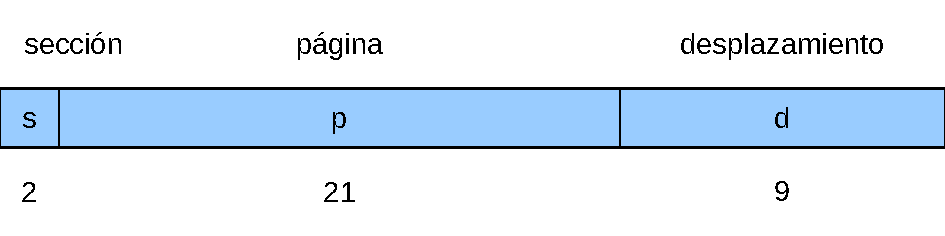
\includegraphics[width=0.8\textwidth]{media/C16_paginación/dirección_virtual_vax.pdf}
\caption{}
\end{figure}

El espacio de direcciones de un proceso estaba dividido en 3 secciones.
Los 2 bits de orden más alto \emph{s} de las direcciones virtuales se
utilizaban para indicar la \textbf{sección}. Cada \textbf{sección}
estaba dividida en \textbf{páginas} de 512 bytes, por lo que los
siguientes 21 bits de las direcciones virtuales \emph{p} eran utilizadas
para seleccionar la \textbf{página} concreta.

Dividiendo el espacio de direcciones de esta manera, el sistema
operativo podía mantener secciones sin utilizar mientras no fueran
necesarias. Esto era importante, puesto que la \textbf{tabla de páginas}
de una \textbf{sección} tenía un tamaño de 8 MiB.

\subsection{Paginación jerárquica de N
niveles}\label{_paginaciuxf3n_jeruxe1rquica_de_n_niveles}

En general, en la \textbf{paginación jerárquica} de \emph{n} niveles el
\textbf{número de página} \emph{p} de cada dirección virtual es dividido
en \emph{n} números: \{ \emph{p}\textsubscript{1},
\emph{p}\textsubscript{2}, \emph{p}\textsubscript{3}, \ldots,
\emph{p\textsubscript{N}}\}, donde:

\begin{enumerate}
\def\labelenumi{\arabic{enumi}.}
\item
  \emph{p}\textsubscript{1} se utiliza para indexar la \textbf{tabla de
  páginas externa} ---también llamada \textbf{directorio de páginas}{} o
  \textbf{tabla de páginas de nivel 0}{}--- cuya dirección conoce la CPU
  mediante el \textbf{PTBR}. La entrada obtenida de esta manera,
  contiene la dirección en la memoria física de una porción de la
  \textbf{tabla de páginas} en el siguiente nivel ---el nivel 1---.
\item
  \emph{p}\textsubscript{2} se utiliza para indexar la \textbf{tabla de
  páginas de nivel 1}. E, igualmente, la entrada así obtenida contiene
  la dirección en la memoria física de una porción de la \textbf{tabla
  de páginas} en el siguiente nivel ---el nivel 2---.
\item
  El proceso continúa hasta que \emph{p\textsubscript{N}}, se utiliza
  para indexar la \textbf{tabla de páginas de nivel N-1}, con la que se
  obtiene el \textbf{número de marco} que es utilizado, finalmente, para
  generar la dirección física al combinarlo con el desplazamiento
  \emph{d} de la dirección virtual.
\end{enumerate}

Como se puede ver, resolver una dirección virtual necesita tantos
accesos a la memoria como niveles hay en la jerarquía.

Debido a que la traducción funciona desde las \textbf{tablas de páginas}
de nivel superior ---nivel 0--- hacia las de nivel inferior ---nivel
\emph{N} - 1--- a esta estructura también se la conoce como
\textbf{tabla de páginas directa}{}.

Los procesadores \{decalpha\} y \{mips\} utilizan una variante
denominada \textbf{tabla de páginas virtualizada}{}. En este esquema, el
último nivel de la \textbf{paginación jerárquica}, aunque esté en marcos
separados en el espacio de direcciones físico, se mapea de manera
continua en el espacio de direcciones virtual del proceso.

Así, si la consulta a la \textbf{TLB} falla, se indexa la \textbf{tabla
de páginas} directamente con direcciones virtuales usando el
\textbf{número de página} completo. Esta consulta conlleva la traducción
de la dirección virtual de la entrada indexada, que puede estar en la
\textbf{TLB}. Si no es así, se pasa a recorrer la \textbf{tabla de
páginas} desde el nivel 0 y usando direcciones físicas.

Existen algunos procesadores que utilizan más de dos niveles. Por
ejemplo, los procesadores x86-64 utilizan un esquema de 4 niveles de
paginación. Cada \textbf{página} es de 4 KiB ---como en el resto de la
familia x86--- pero como cada entrada en la \textbf{tabla de páginas} es
de 8 bytes ---con el fin de poder almacenar direcciones de 64 bits--- en
cada una caben 512 entradas, por lo que los \textbf{números de página}
de cada nivel necesitan 9 bits. Eso significa que de las direcciones
virtuales se utilizan actualmente 48 bits ---resultado de multiplicar 4
niveles por 9 bits cada uno más 12 bits de desplazamiento--- aunque el
límite de la arquitectura para las direcciones virtuales sea de 64 bits.

\subsection{Tiempos de acceso a la
memoria}\label{_tiempos_de_acceso_a_la_memoria_2}

La \textbf{paginación jerárquica} aumenta el número de accesos
necesarios para consultar la \textbf{tabla de páginas}. Es decir,
mientras que para consultar una \textbf{tabla de páginas lineal} solo
necesitamos un acceso a la memoria, para obtener una dirección fisica en
la \textbf{paginación jerárquica} de \emph{n} niveles necesitamos
\emph{n} accesos a la memoria. Por tanto, el \textbf{tiempo de acceso
efectivo} \(T_text(em)\) en un sistema sin \textbf{TLB} es:

\[T_"em" = (n+1)*T_"m"\]

porque, además de los \emph{n} accesos para consultar la \textbf{tabla
de páginas} y obtener la dirección física, es necesario ejecutar la
operación solicitada en la memoria física.

Como en el \hyperref[_tiempos_de_acceso_a_la_memoria]{Tiempos de acceso
a la memoria}, cuando el sistema dispone de \textbf{TLB}, el
\textbf{tiempo de acceso efectivo} \(T_text(em)\) anterior corresponde
al caso en el que la dirección virtual no está en la \textbf{TLB}.
Mientras que, en caso contrario, el \textbf{tiempo de acceso efectivo}
es \(T_text(em)=T_text(m) + T_text(TLB)\).

Siguiendo los mismos pasos que en el
\hyperref[_tiempos_de_acceso_a_la_memoria]{Tiempos de acceso a la
memoria}, para obtener una estimación de \(T_text(em)\) en base a la
probabilidad \(p_text(TLB)\) de que las direcciones virtuales
consultadas estén en la \textbf{TLB}, obtenemos el siguiente resultado:

\[{:(T_"em", =, (1-p_"TLB")*((n+1)*T_"m" + T_"TLB") + p_"TLB"*(T_"m" + T_"TLB")),
    (    , =, ((1-p_"TLB")*n+1)*T_"m" + T_"TLB"\qquad\qquad\qquad\qquad\qquad\ \ ):}\]

Esta expresión se puede simplificar si consideramos que
\(T_text(TLB) ll T_text(m)\):

\[{:(T_"em", =, (1-p_"TLB")*(n+1)*T_"m" + p_"TLB"*T_"m"),
    (    , =, ((1-p_"TLB")*n+1)*T_"m"\qquad\qquad\qquad):}\]
